\section{Pseudonymisierung}

\label{sec_basics_pseudonymity}

Ein Pseudonym\footnote{
	Ursprünglich aus dem Griechischen stammend: \textit{pseudonumon} - falsch benannt.
} bezeichnet nach \cite{pfitzmann2010} einen Identifikator eines Subjekts ungleich seinem echten Bezeichner. Im BDSG wird zusätzlich noch der \glqq Zweck [eines Pseudonyms], die Bestimmung des Betroffenen auszuschließen oder wesentlich zu erschweren\grqq{}\footnote{
  BDSG, § 3, Absatz 6a.
} ergänzt. Beispiele für Pseudonyme lassen sich in verschiedensten Bereichen finden: E-Mail-Adressen, Sozialversicherungsnummern oder auch Autoren, die unter einem Pseudonym ihre Schriften veröffentlichen.

Nach \cite{pfitzmann1990} lassen sich unterschiedliche Arten von Pseudonymen unterscheiden. Eine Eigenschaft, die zur Unterscheidung herangezogen werden kann, ist die (Un-)Kenntnis des Zusammenhangs zwischen dem Pseudonym und dem zugehörigen Subjekt (auch Pseudonymhalter genannt) zu Beginn seiner Verwendung. Dieser Zusammenhang wird als Zuordnungsvorschrift bezeichnet und kann beispielsweise als Funktion oder in Tabellenform vorliegen.\\
Hier kann zwischen öffentlichen, nicht-öffentlichen und anonymen Pseudonymen unterschieden werden. Ein öffentliches Pseudonym ist beispielsweise die Telefonnummer einer Person, die von Beginn an im öffentlichen Telefonbuch mit der Identität der Person verknüpft ist. Eine Kontonummer zu einem Bankkonto, dessen Inhaber bei der Kontoeröffnung nur der Bank und ihm selbst bekannt ist, bildet ein nicht-öffentliches Pseudonym -- die Zuordnung ist nur wenigen Stellen bekannt. Ein anonymes Pseudonym ist zu Beginn nur dem Besitzer bekannt. Ein Beispiel bildet ein selbstgewählter Benutzername in einem Webforum ohne Hinterlegung identifizierender Merkmale wie Klarname oder Adresse.\\
Die beschriebene Eigenschaft eines Pseudonyms kann sich im Laufe der Zeit ändern, wenn Informationen über den Zusammenhang zwischen Pseudonym und zugehörigem Subjekt veröffentlicht werden.

In enger Verbindung mit Pseudonymen steht auch der Begriffe der Verkettbarkeit. 
Verkettbarkeit bezeichnet dabei die Eigenschaft, dass ein Außenstehender mit hoher Wahrscheinlichkeit entscheiden kann, ob zwei Objekte in einem System unabhängig sind \cite{pfitzmann2010}.

\begin{figure}[]
    \centering
        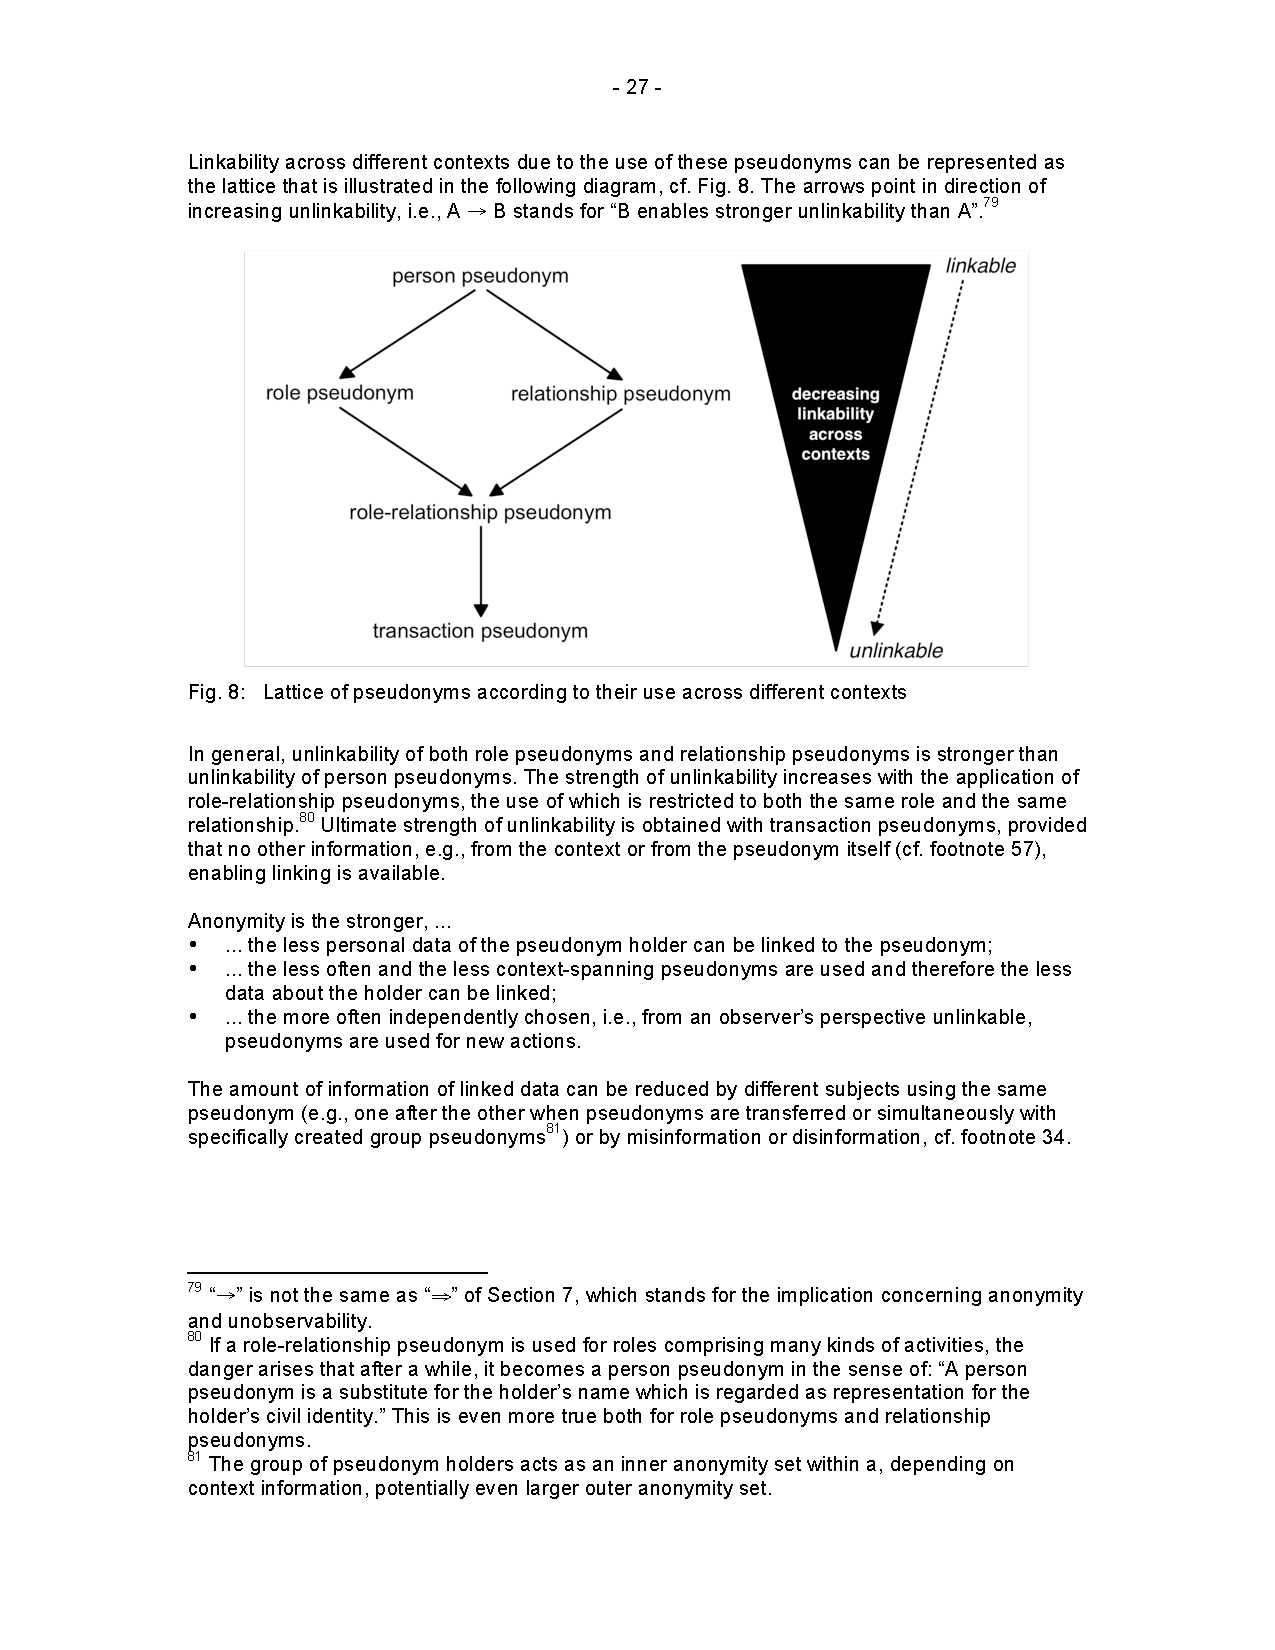
\includegraphics[clip, trim=0cm 16.5cm 0cm 4cm, width=1.00\textwidth]{img/pseudonym_lattice_excerpt.pdf}
    \caption{Pseudonym-Verband entsprechend ihrer Nutzung in verschiedenen Kontexten. Entnommen aus \cite{pfitzmann2010}.}
    \label{fig:lattice_pseudonym}
\end{figure}

Auf Basis dieser Eigenschaft lassen sich nun ebenfalls verschiedene Arten von Pseudonymen ausmachen, die sich durch Nutzung des Pseudonyms in verschiedenen Kontexten unterscheiden: Personen-, Rollen-, Beziehungs-, Rollen-Beziehungs- oder Transaktionspseudonym sind mögliche Ausprägungen dieser Eigenschaft. Eine Übersicht über diese Pseudonymarten und deren Zusammenhang zur Verkettbarkeit ist Abbildung \ref{fig:lattice_pseudonym} zu entnehmen.\\
Personenpseudonyme beschreiben Pseudonyme, wie beispielsweise die Sozialversicherungsnummer, die stellvertretend für die eindeutige Identität des Subjekts in der Gesellschaft stehen. Ereignisse, die mit solchen Pseudonymen verbunden sind, lassen sich über die gesamte Gültigkeitsspanne des Pseudonyms verketten. \\
Rollen-, Beziehungs- und Rollen-Beziehungspseudonyme stellen Pseudonyme dar, die das Subjekt nur in einer besonderen Funktion oder mit einem bestimmten Kommunikationspartner bzw. in der Kombination beider Möglichkeiten nutzt. Ein Beispiel hierfür wäre eine E-Mail-Adresse wie \textit{administrator@unternehmen.de} in einem Unternehmen, die nicht das Subjekt als solches sondern nur in seiner Rolle in dem Unternehmen beschreibt. Ereignisse verbunden mit diesen Pseudonymarten lassen sich nur in bestimmten Kontexten, jedoch nicht über Kontextgrenzen hinweg verknüpfen. Beispielsweise könnten zwei Kommunikationspartner mit derselben Person kommunizieren, ohne dies feststellen zu können, wenn die Person ihnen gegenüber unter unterschiedlichen Beziehungspseudonymen auftritt.\\
Transaktionspseudonyme stellen die stärkste Form der Unverkettbarkeit da. Bei dieser Art von Pseudonymen wird für jedes Ereignis ein neues Pseudonym verwendet, das daher nur ein einziges Mal auftritt und Verkettbarkeit verhindert.

%\tbc{Abgrenzung zur Anonymität sinnvoll?}

%\tbc{Ist der \glqq Schnitt\grqq{} zwischen Kapitel 2 und 3 hier sinnvoll?}